\subsection{Dynamical results}
\label{sec:results_dynamics}

The central dynamical question is whether self-consistent electrostatics change the failure modes of interatomic potentials under nonequilibrium trajectories. The evidence points to a mixed answer: charge-aware models can improve static ranking, but their dynamical effect remains strongly dependent on the target system and the stress protocol.

\subsection{Reference system stability: OpenREACT}
On the OpenREACT reference system, all model families, \texttt{short\_range}, \texttt{static\_charge}, and \texttt{self\_consistent}, remain numerically stable over short horizons ($300$ steps). Under the more demanding protocol ($2400$ steps at $\Delta t = 0.50$), the charge-aware branches show smaller potential-energy drift than the short-range baseline. The \texttt{static\_charge} and \texttt{self\_consistent} variants, however, remain nearly tied. Charge-aware dynamics are therefore active on the bridge system, while explicit self-consistency does not separate itself from a fixed-partial-charge reference in this regime.

\subsection{Hierarchy reversal: Transition1x}
Transition1x provides a stricter test of dynamical robustness. Although the static results in Section \ref{sec:results_static} favour the charge-aware families, the dynamical stress tests reverse that hierarchy. Under the harshest protocol, the \texttt{short\_range} baseline is substantially more stable than both charge-aware branches. For frames $64$ and $128$, the \texttt{short\_range} model never crosses the selected force or drift thresholds within the $2400$-step horizon, whereas both charge-aware branches cross them before step $2251$.

Bond-network observables clarify that reversal. The onset of local structural anomalies, measured by bond-threshold crossings and coordination-number reduction, is nearly synchronized across all three families. The divergence appears only in the post-onset regime: \texttt{short\_range} preserves a larger stability margin after the initial bond-network rearrangement, whereas the charge-aware families enter the degraded regime earlier. Electrostatic corrections therefore remain compatible with improved static force accuracy while still introducing additional sensitivity once the geometry becomes strongly distorted.

\subsection{Frame-selective synchronized collapse: SPICE}
SPICE reveals a different organization of failure. Unlike Transition1x, the SPICE trajectories do not show a clear family-level threshold hierarchy. Instead, the dominant signal is frame selectivity: on the most fragile trajectories, such as frame $64$, all three families undergo synchronized bond-network collapse by step $150$, whereas on more stable frames all families remain intact across the full horizon. For this system, the intrinsic susceptibility of specific trajectories to collective bond failure therefore dominates over inter-family differences in electrostatic representation.

\subsection{Final target plateau: CL-20/HMX}
The final energetic-material benchmark sharpens the main dynamical boundary. A sequence of progressively stronger protocols was applied to the CL-20/HMX data: short smoke trajectories, a longer horizon test, stress rollouts, threshold-aware stress, later-frame reaction-progress trajectories, a dense multiframe ensemble, and finally a focused key-bond survival comparison on the most sensitive frames. Across this ladder, the leading source of variation is the starting frame rather than the model family, and the new frame-versus-family dominance summary makes that statement quantitative rather than impressionistic.

The static hierarchy from Section \ref{sec:results_static} therefore does not propagate into a clear dynamical hierarchy under the current nonequilibrium protocols. In the threshold-aware stress analysis, all three families cross the potential-drift threshold at nearly identical times within each frame: around step $1631$ for frame $64$, around $1560$ for frame $128$, and around $1636$--$1637$ for frame $192$. Force and total-energy thresholds remain untriggered across this comparison.

The dense frame ensemble reinforces the same interpretation. Frames $32$, $64$, and $160$ are visibly more fragile than the others in molecular-integrity space, yet within a fixed frame the three families remain nearly indistinguishable.

The focused key-bond survival comparison gives the clearest chemical view of this boundary. On frame $32$, all three families finish with the same molecular-integrity fraction ($0.333$), the same retained C--N bond fraction ($0.910$), the same retained N--O bond fraction ($0.827$), and the same first molecular-integrity crossing below $0.5$ (step $390$), with the potential-drift threshold appearing at step $1117$--$1118$. Frame $64$ is similar: all three families end at molecular integrity $0.286$, retained C--N $0.912$, retained N--O $0.553$, and the same first integrity crossing at step $390$. Even on frame $160$, where the molecular-integrity crossing shifts earlier to step $360$--$370$, the family-level spread remains negligible (Figure \ref{fig:cl20_hmx_target_dynamics_keybond_survival}).

The dominance summary compresses that pattern into one quantitative comparison. For the final molecular-integrity and retained-bond endpoints, the mean spread across families within a fixed frame is exactly zero, while the same family's spread across frames reaches $0.464$ in final molecular integrity and $0.362$ in retained N--O fraction (Table \ref{tab:cl20_hmx_frame_family_dominance}). Even the event-onset metrics follow the same ordering: the mean spread across frames is about $8\times$ larger than the family spread for the first integrity crossing and about $184\times$ larger for the first drift-threshold step.

A dedicated multiseed nitro-focus analysis on frame $160$ sharpens the same point rather than reversing it. Averaged over $15$ variants spanning \texttt{short\_range}, \texttt{static\_charge}, \texttt{self\_consistent}, and two damped self-consistent ablations, the retained nitro N--O fraction is $0.444$ for \texttt{short\_range} and $0.463$ for every charge-aware family, while the nitro-motif integrity converges to the same mean value ($0.148$) for all five families and the first motif-integrity crossing below $0.5$ remains tightly clustered around steps $1647$--$1663$.

We also tested two stronger charge-aware modifications targeted directly at this boundary: a train-matched self-consistent comparison that removes the rollout-time damping used in the earlier horizon test, plus a stability-gated adaptive branch that modulates the self-consistent update step size on the fly. The train-matched comparison is especially important because it closes the most obvious method objection.

On frame $160$, restoring the static-side self-consistent settings (\texttt{charge\_iterations} $=4$, full-step updates, no rollout-only gate) does not create a new family-level win. Instead, it leaves the main endpoint picture essentially unchanged while shifting the onset metrics only modestly: the first potential-drift threshold moves from step $1067$ in the rollout-stabilized self-consistent family to step $1058$ in the train-matched family, the final molecular-integrity fraction remains $0.583$ in both cases, and retained N--O fraction changes slightly from $0.903$ to $0.887$. The same train-matched comparison also advances the first $0.70$ bond-threshold crossing from $433.3$ to $363.3$, which weakens rather than strengthens the hypothesis that the earlier negative result was caused purely by rollout-time damping.

In other words, the absence of a family-level dynamic gain survives the most direct configuration-fairness check we can presently perform on the fragile-frame target.

The new fragile-frame analysis makes the remaining dynamic signal more specific. The earlier failure-manifold comparison showed that the train-matched branch was the only self-consistent variant with any clear positive signal on the real target, but the denser failure-window analysis around frames $56$, $64$, and $72$ changes the interpretation of that signal.

This denser comparison rejects a broad onset-gain story: averaged over five seeds, train-matched \texttt{self\_consistent} reaches the first $0.70$ bond-threshold crossing earlier than \texttt{static\_charge} on all three frames ($-12$ steps on frame $56$, $-34$ on frame $64$, and $-18$ on frame $72$). The positive signal instead reorganizes around endpoint survival.

On frame $64$, train-matched \texttt{self\_consistent} still improves the final molecular-integrity fraction from about $0.343$ for \texttt{static\_charge} to about $0.426$, and on frame $72$ it improves final molecular integrity from about $0.774$ to about $0.832$ while also delaying the first integrity crossing by about $195$ steps and slightly improving final nitro N--O survival. Frame $56$ remains unfavorable, with train-matched \texttt{self\_consistent} worse than \texttt{static\_charge} on final integrity and nitro survival.

Figure \ref{fig:cl20_hmx_failure_window} and Table \ref{tab:cl20_hmx_failure_window} compress that result into the most direct comparison. The clearest local gain is frame $72$, where the train-matched branch improves final integrity relative to both \texttt{static\_charge} and \texttt{short\_range}, while frame $64$ still shows a smaller endpoint gain and frame $56$ shows no gain at all. The fragile-window analysis therefore sharpens the dynamic conclusion in a more constructive way than the earlier broad ladders alone: on the real CL-20/HMX target, the strongest positive signal is not a generic onset delay but a narrow endpoint-survival gain window around frames $64$--$72$.

Even this stronger window remains local rather than global, because it does not extend across the broader fragile manifold and does not establish a robust family-level hierarchy over the final target as a whole.

The adaptive-gated branch remains informative for a different reason. On the same frame-$160$ horizon test, neither gated modification improves the existing charge-aware drift-threshold plateau in a meaningful structural sense, and the adaptive-gated variant preserves the same molecular-integrity outcome while entering a substantially more expensive rollout regime.

A matched profiled comparison now makes the family-level cost ordering explicit on that frame: \texttt{short\_range}, \texttt{static\_charge}, and train-matched \texttt{self\_consistent} all remain within the same early-event band, while rollout costs still rise from about $20$ s to $42$ s to $112$ s before the adaptive-gated branch reaches about $190$ s without creating a better endpoint hierarchy (Figure \ref{fig:cl20_hmx_target_adaptive_gate_cost}).

The submission package includes a dedicated QEq-versus-failure bridge table, a frame-versus-family dominance summary, a train-matched frame-$160$ dynamics table, a frame-$160$ adaptive-gate cost-versus-outcome table, a threshold-aware fragile-frame summary, and a failure-manifold summary to make the implication explicit: the charge-aware branches remain measurably active in the static diagnostics, yet within a fixed CL-20/HMX frame the dominant variation in final integrity and key-bond survival still comes from frame choice rather than from family choice, while progressively more elaborate charge-aware branches can impose progressively larger rollout cost without producing a new event hierarchy or a better structure-survival endpoint.

The real target therefore supports a stronger statement than drift alone would allow: key-bond survival, nitro-motif survival, and fragment-level integrity remain dominated by frame selection rather than by the choice among \texttt{short\_range}, \texttt{static\_charge}, and \texttt{self\_consistent}, even though the train-matched branch can open a narrow local endpoint-survival gain window on the most fragile frames.

\subsection{Summary of dynamical findings}
Taken together, the dynamical evidence defines a clear boundary for charge-self-consistent potentials. The public systems support a measurable electrostatic effect and substantial heterogeneity across surrogate targets, but they do not support a universal dynamical improvement. Transition1x shows that charge-aware families can become less stable than the short-range baseline after comparable early rearrangement, whereas SPICE shows that some trajectories collapse synchronously across all three families before any hierarchy can emerge. The final CL-20/HMX benchmark goes further: under the present nonequilibrium protocols, degradation is primarily frame-dependent rather than family-dependent, even when evaluated by key-bond survival and molecular-integrity observables. These findings support CSC-MACE as a physically motivated architecture while defining the stabilization problem that remains unresolved on the final target.

\begin{figure}[t]
    \centering
    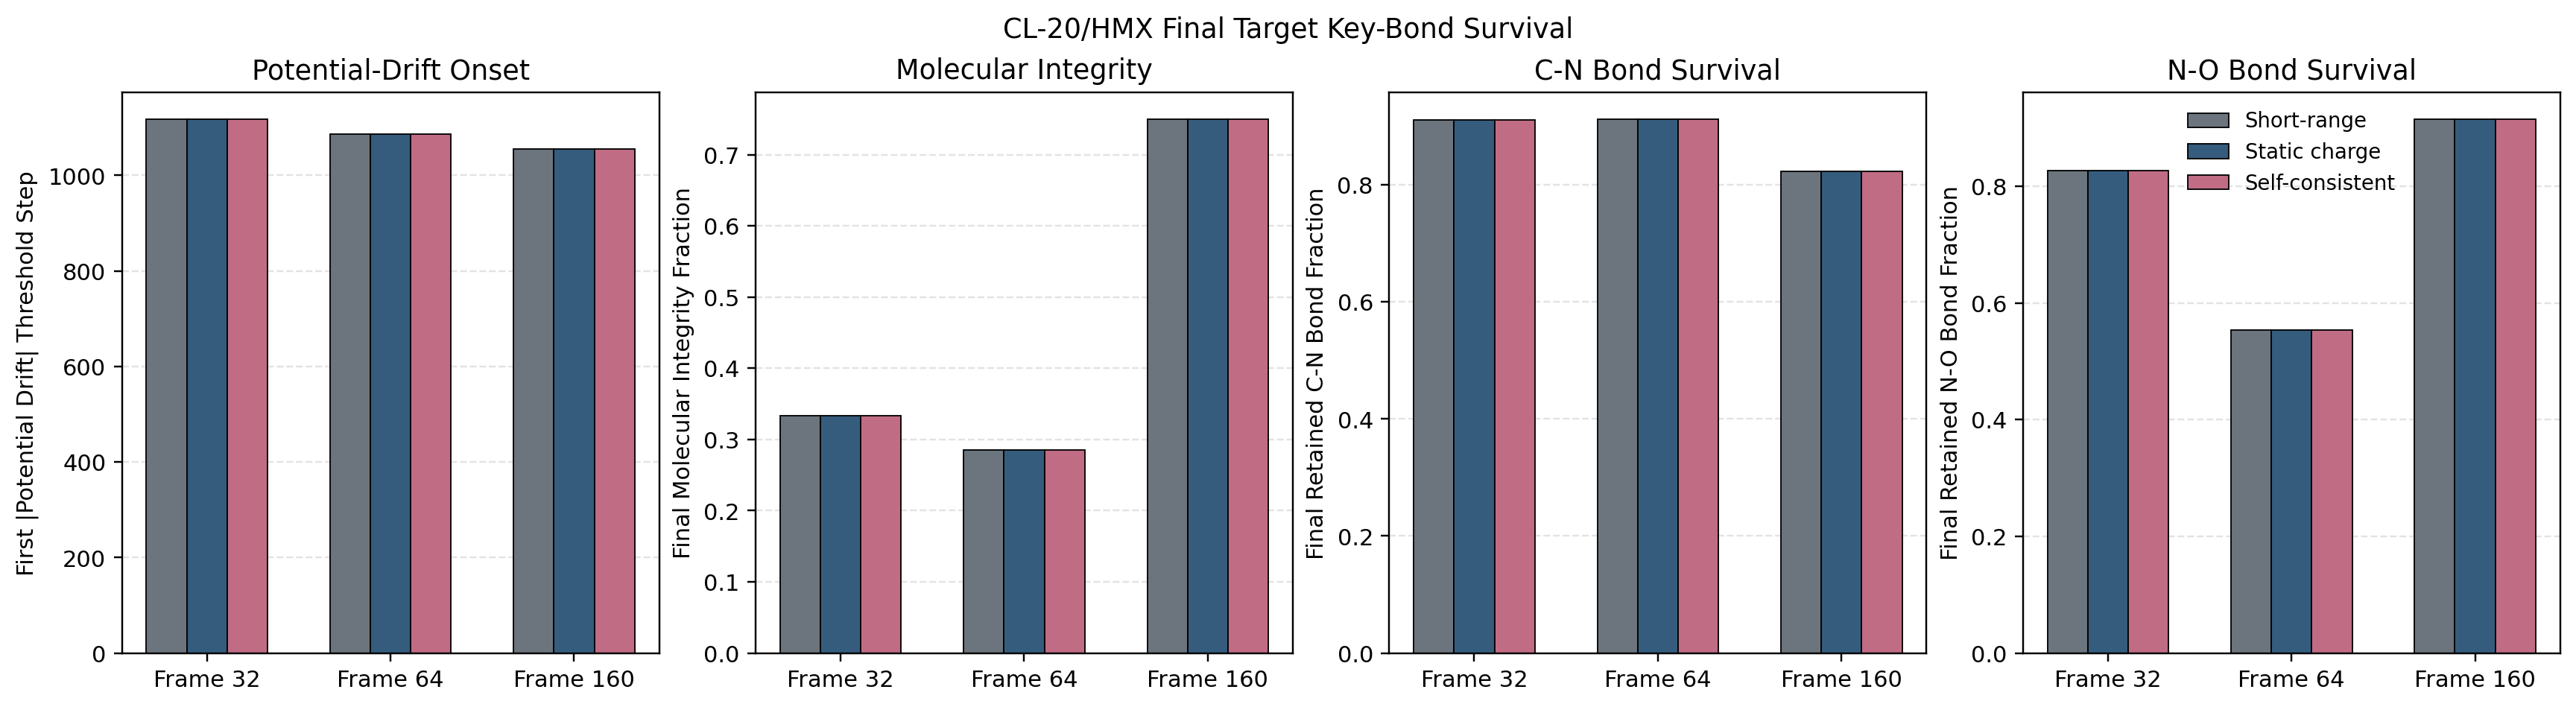
\includegraphics[width=\linewidth]{figs/cl20_hmx_target_dynamics_keybond_survival.png}
    \caption{CL-20/HMX final-target focused key-bond survival comparison on the most sensitive frames $32$, $64$, and $160$. Potential-drift onset, molecular integrity, and C--N / N--O bond-family survival all vary substantially across starting frames, but remain nearly unchanged across the three model families within each frame.}
    \label{fig:cl20_hmx_target_dynamics_keybond_survival}
\end{figure}

\input{../results/target/cl20_hmx_frame_family_dominance.tex}

\begin{figure}[t]
    \centering
    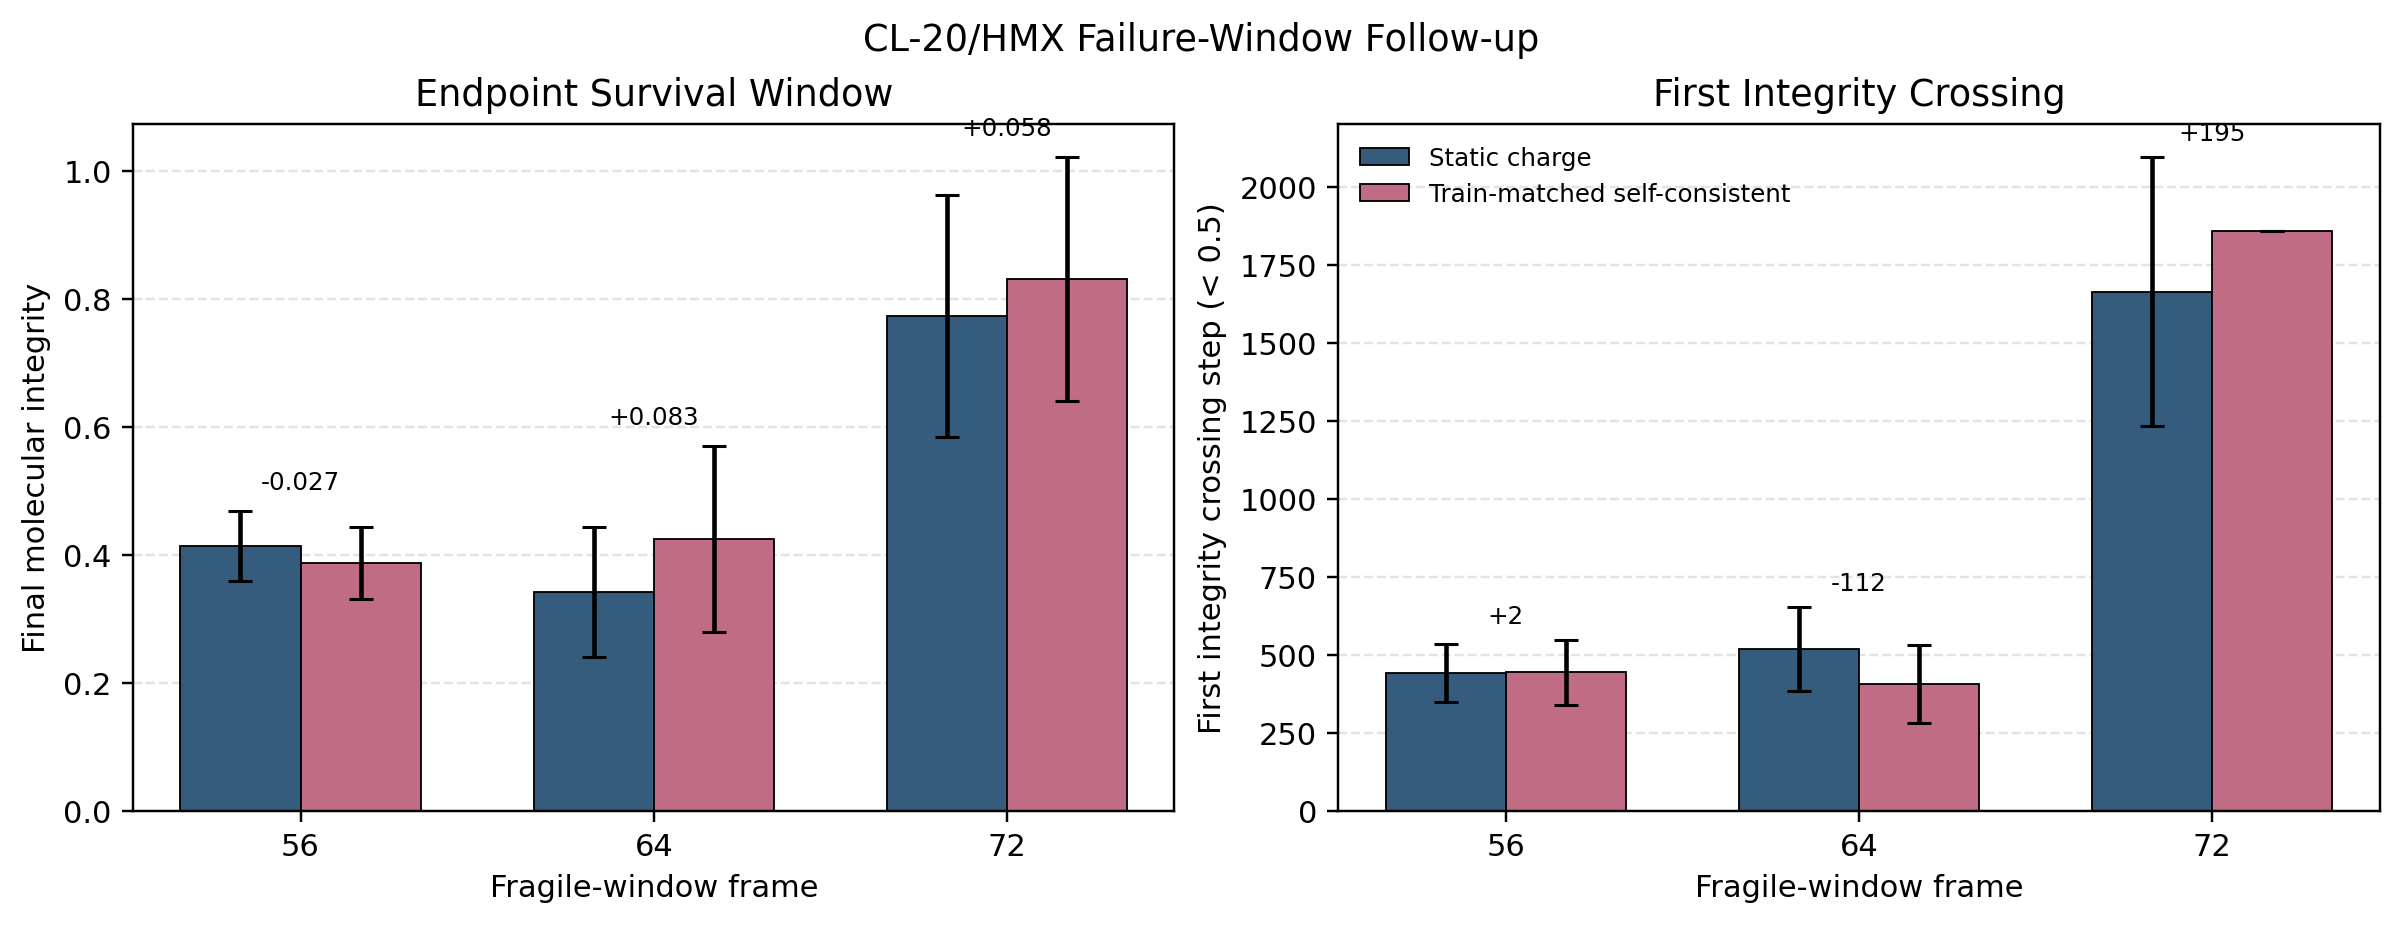
\includegraphics[width=\linewidth]{figs/cl20_hmx_failure_window.png}
    \caption{Dense CL-20/HMX fragile-window analysis comparing \texttt{static\_charge} against train-matched \texttt{self\_consistent}. The positive dynamic signal is not a broad onset advantage. Instead, endpoint survival improves only in a narrow local window: frame $56$ remains unfavorable, frame $64$ shows a modest final-integrity gain, and frame $72$ shows the clearest combined endpoint benefit.}
    \label{fig:cl20_hmx_failure_window}
\end{figure}

\input{../results/target/cl20_hmx_failure_window_summary.tex}

\begin{figure}[t]
    \centering
    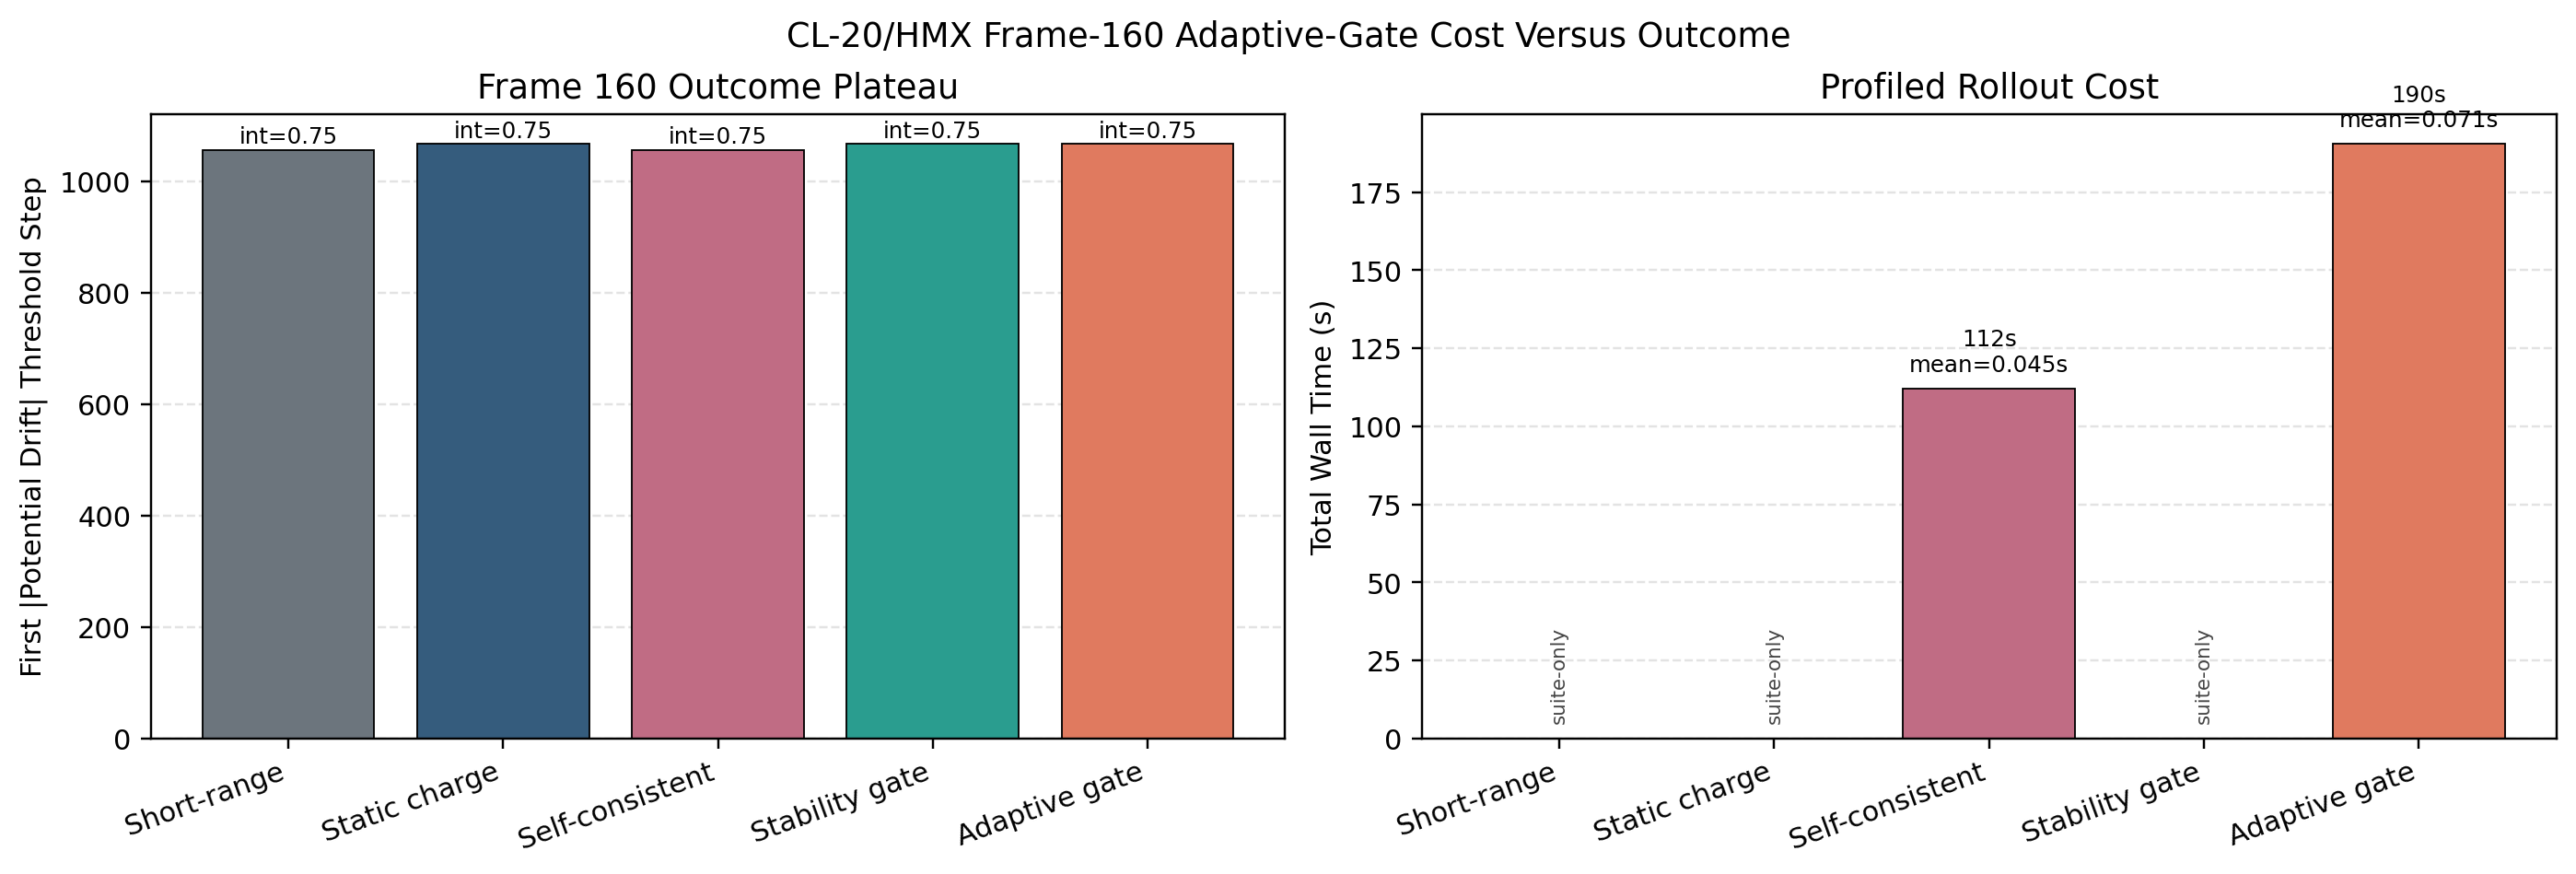
\includegraphics[width=0.95\linewidth]{figs/cl20_hmx_adaptive_gate_cost.png}
    \caption{CL-20/HMX frame-$160$ cost-versus-outcome comparison for the breakthrough charge-aware branches. The stronger gated variants recover the same structure-level outcome and the same charge-aware drift-threshold plateau, but the adaptive-gated branch does so at substantially higher rollout cost than the plain self-consistent branch.}
    \label{fig:cl20_hmx_target_adaptive_gate_cost}
\end{figure}
